\chapter{Phân tích hệ thống}
  \section{Biểu đồ phân cấp chức năng}
    \begin{center}
      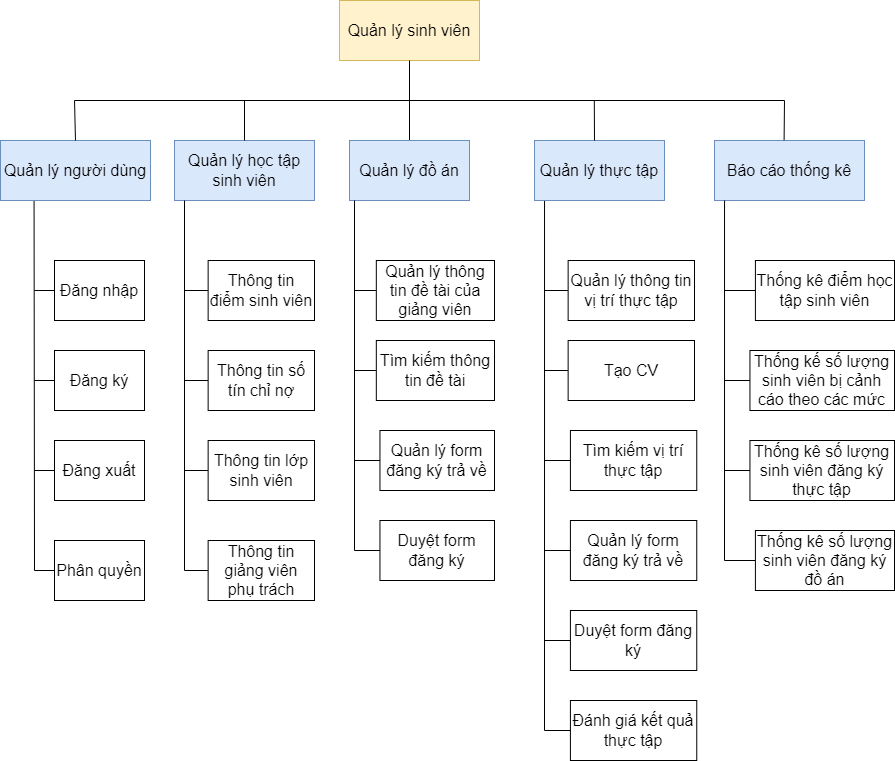
\includegraphics[width=1.05\textwidth]{../drawio/bieudophancapchucnang.drawio.png}
      \begin{figure}
        \centering
        \caption{Biểu đồ phân cấp chức năng}
      \end{figure}
    \end{center}

  \section{Biểu đồ usecase}
    \begin{center}
      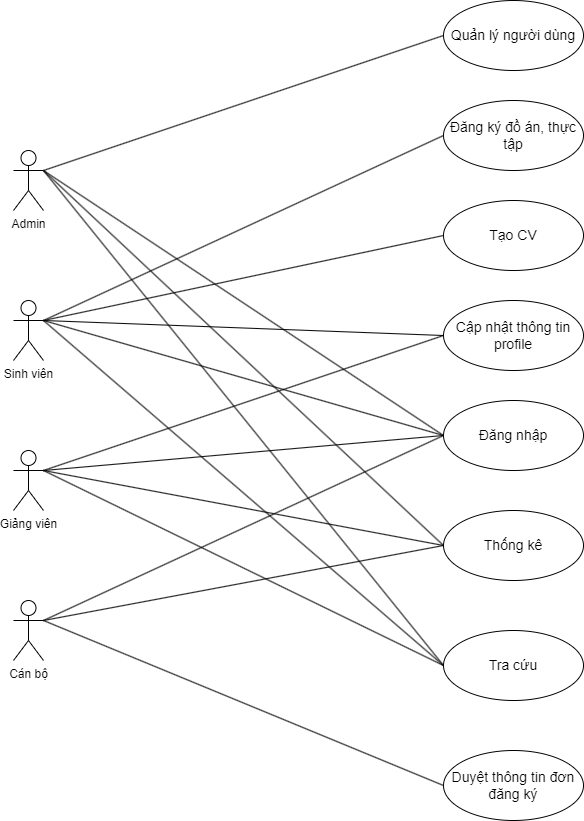
\includegraphics[width=.9\textwidth]{../drawio/usecasee1.png}
      \begin{figure}[h]
        \centering
        \caption{Biểu đồ usecase tổng quát}
      \end{figure}
    \end{center}
    \begin{center}
      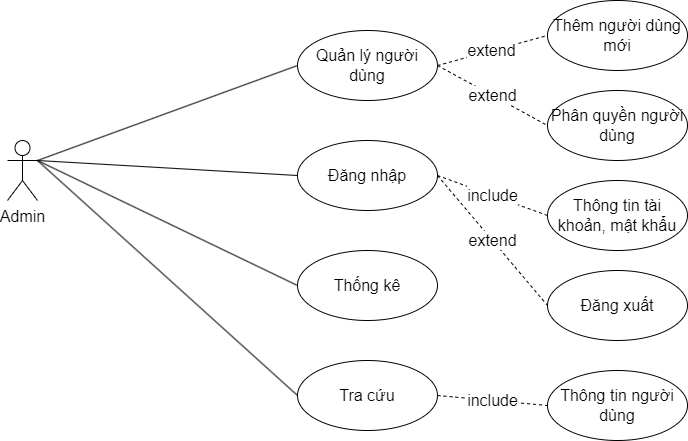
\includegraphics[width=.9\textwidth]{../drawio/usecase22.png}
      \begin{figure}[h]
        \centering
        \caption{Biểu đồ usecase dành cho quản trị viên}
      \end{figure}
    \end{center}
    \begin{center}
      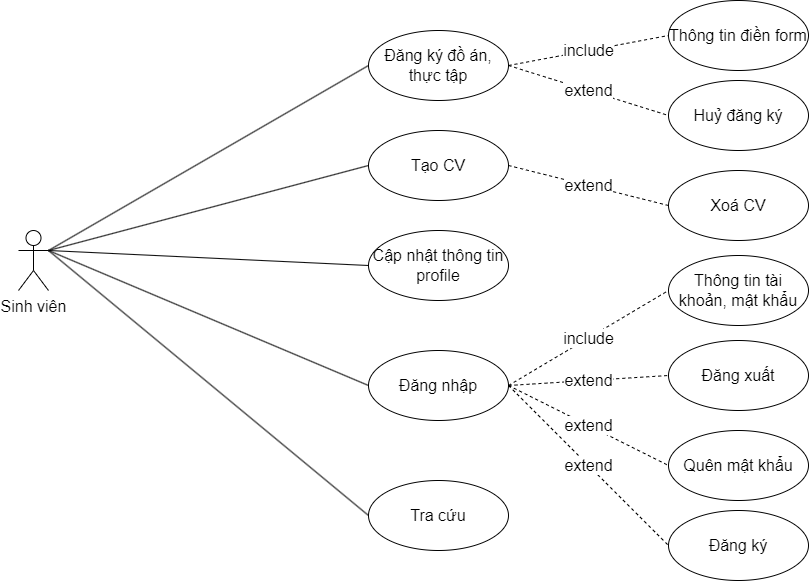
\includegraphics[width=.9\textwidth]{../drawio/usecase33.png}
      \begin{figure}[h]
        \centering
        \caption{Biểu đồ usecase dành cho sinh viên}
      \end{figure}
    \end{center}
    \begin{center}
      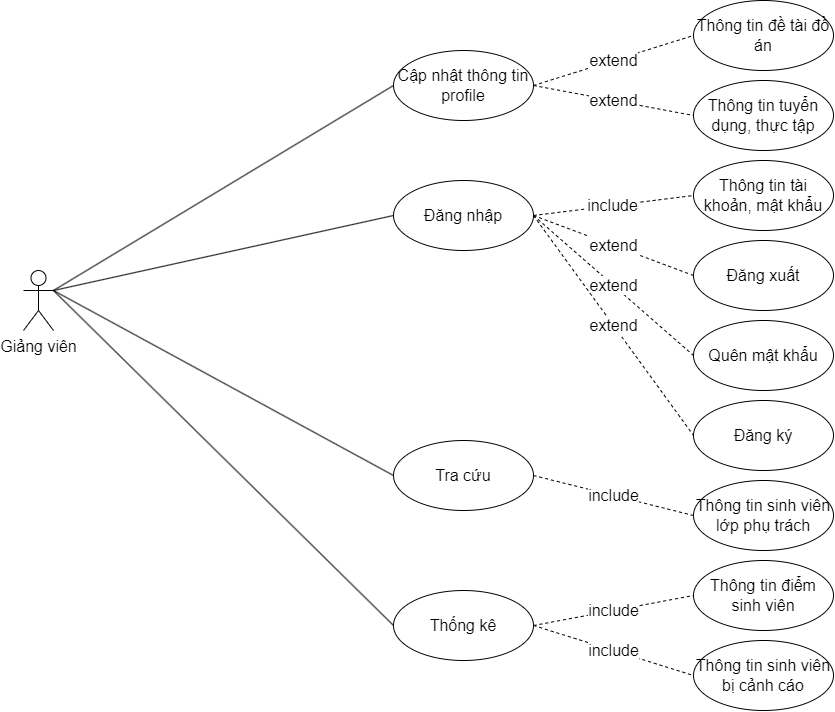
\includegraphics[width=.9\textwidth]{../drawio/usecase44.png}
      \begin{figure}[h]
        \centering
        \caption{Biểu đồ usecase dành cho giảng viên}
      \end{figure}
    \end{center}
    \begin{center}
      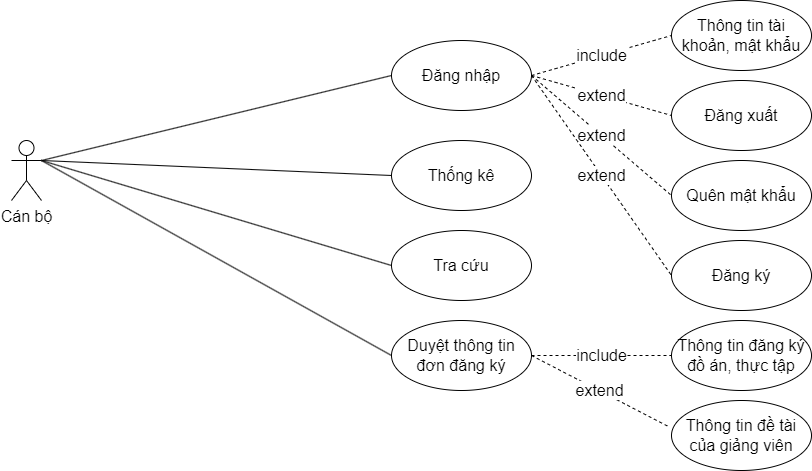
\includegraphics[width=.9\textwidth]{../drawio/usecase55.png}
      \begin{figure}[h]
        \centering
        \caption{Biểu đồ usecase dành cho cán bộ}
      \end{figure}
    \end{center}

  \section{Biểu đồ lớp}
    \begin{center}
      \includegraphics[width=1.2\textwidth]{../out/plantUML/class/class1.png}
      \begin{figure}[h]
        \centering
        \caption{Biểu đồ lớp}
      \end{figure}
    \end{center}